

\begin{frame}{Transformer }
  \begin{itemize}
      \item Encoder-Decoder Deep Learning Architektur für NLP Anwendungen
      \item Basieren auf Attention-Layern
      \item Parallelisierbarkeit zur Performancesteigerung
      \item Encoder wandelt eine Eingabesequenz $(x_1,\ldots,x_n)$ in eine kontinuierliche Übergangsrepräsentation $z=(z_1, \ldots, z_n)$ um
      \item Decoder kann aus Übergangsrepräsentation $z$ eine Ausgabesequenz $(y_1, \ldots, y_n)$ generieren
      \item Decoder ist autoregressiv
  \end{itemize}
\end{frame}

\begin{frame}{Transformer Encoder / Decoder}
  \begin{figure}
    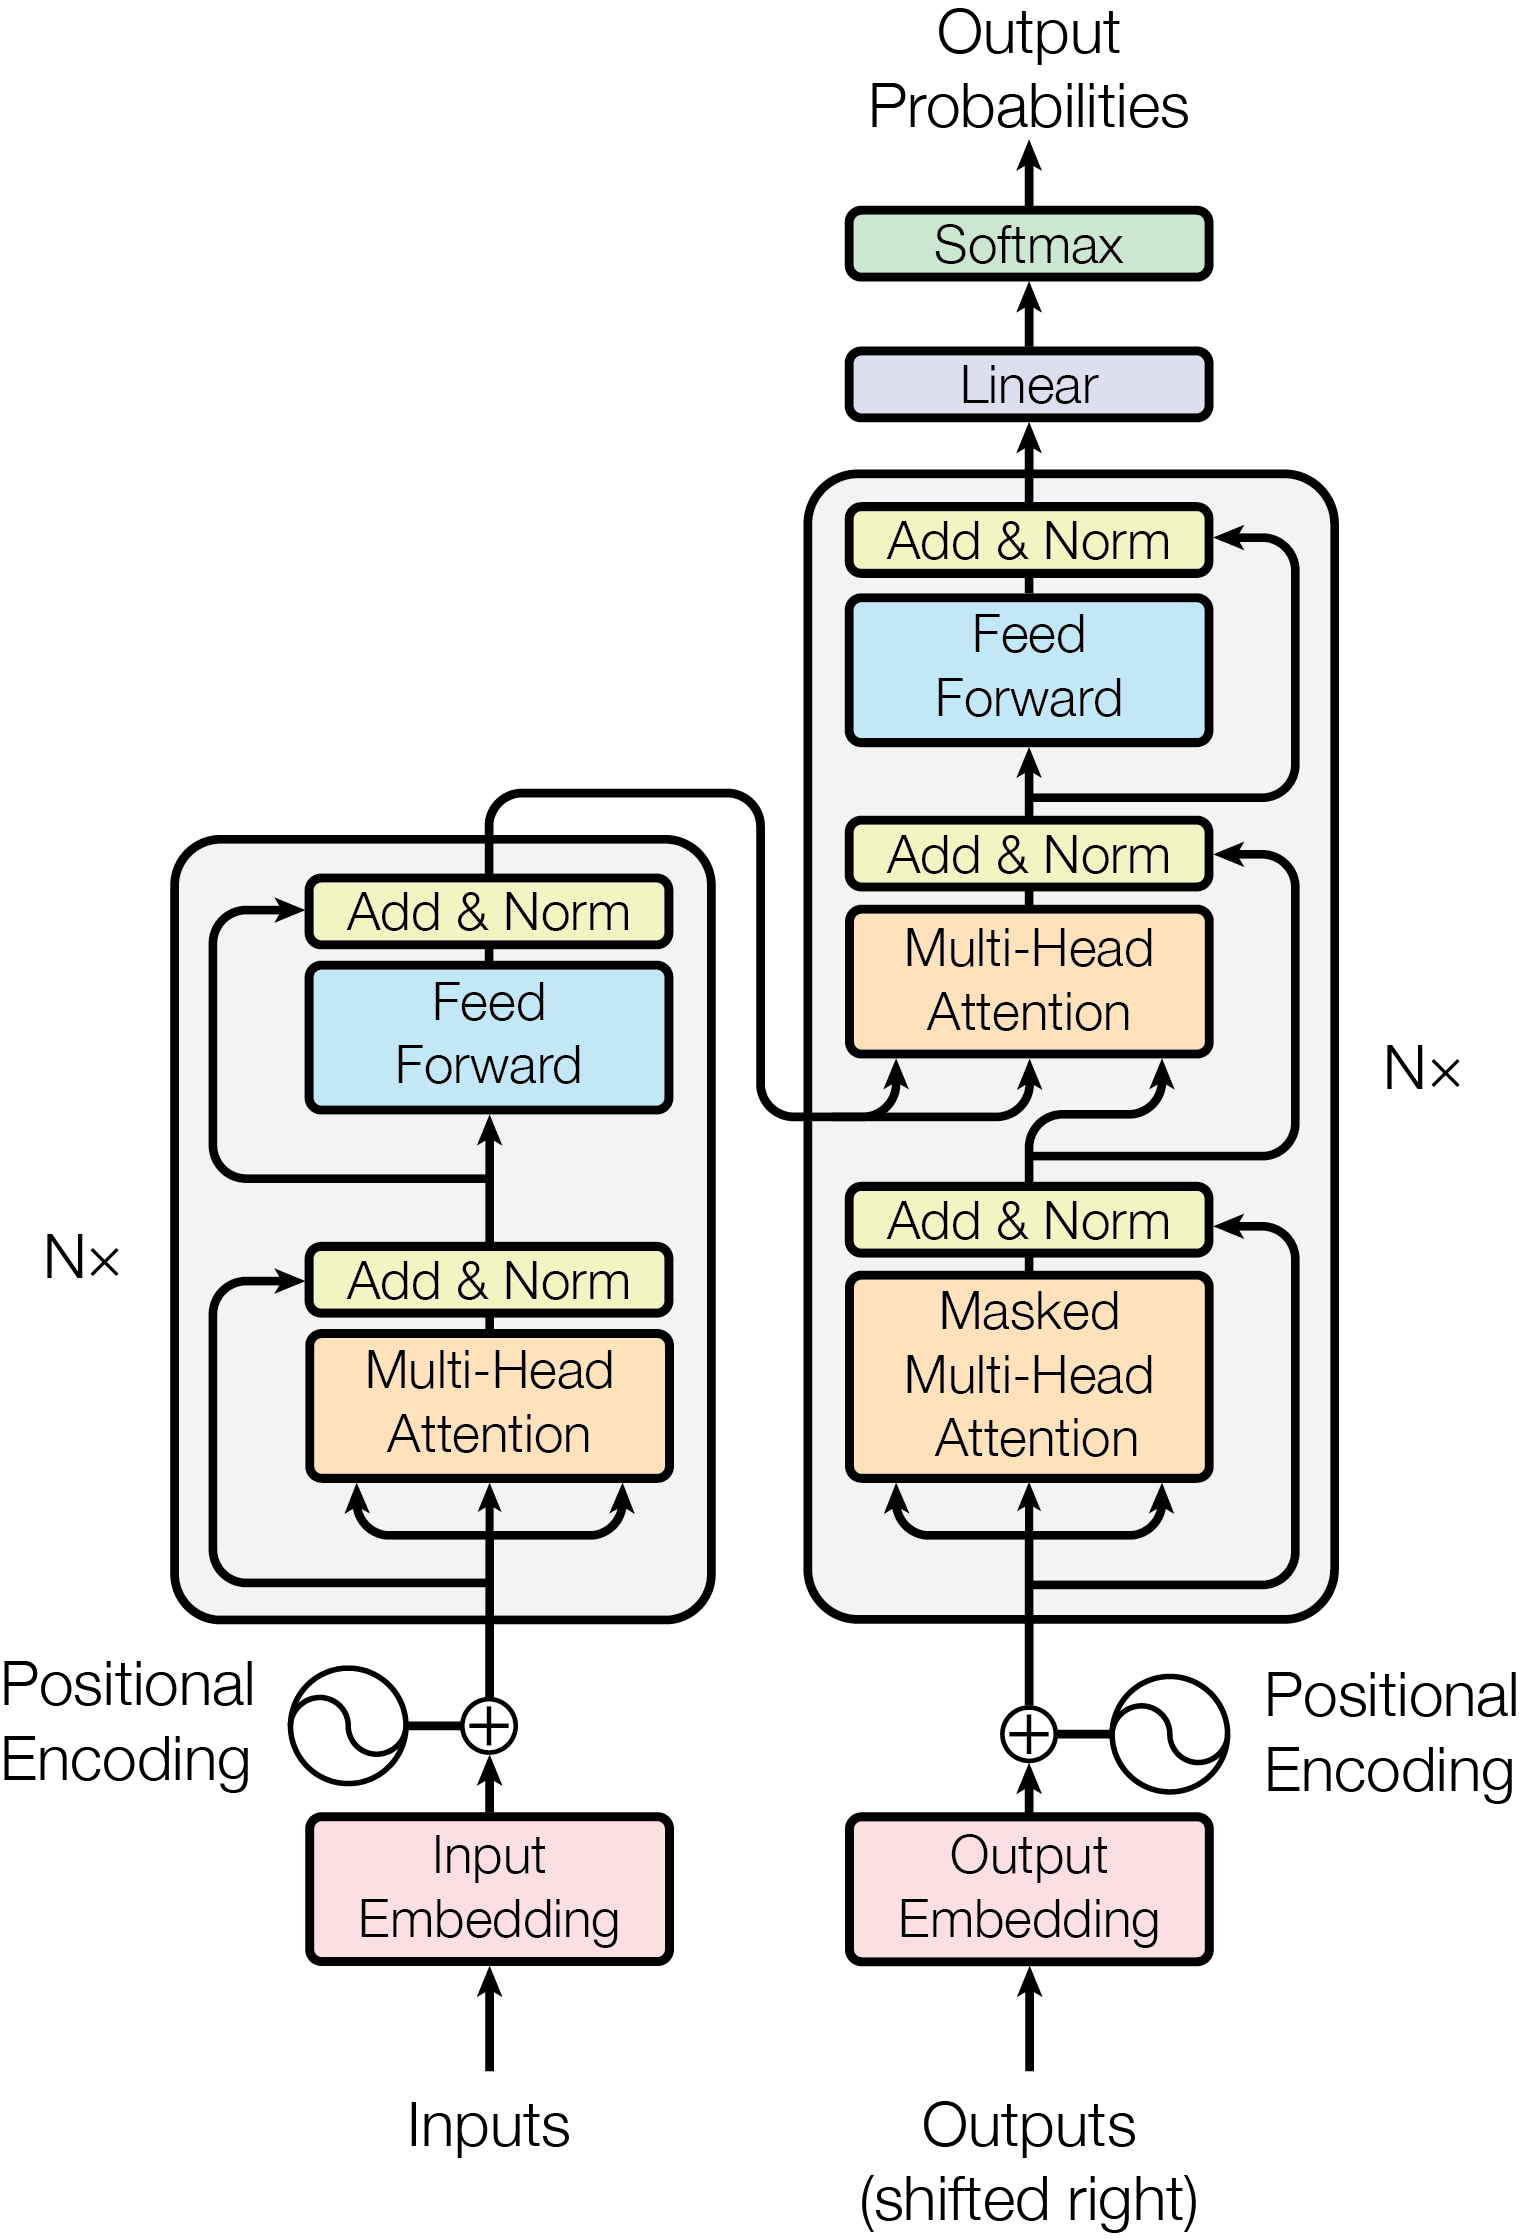
\includegraphics[width=0.25\textwidth]{bilder/Transformer-Encoder-Decoder.png}
    \caption{Transformer Encoder (links) und Transformer Decoder (rechts)}
    \end{figure}
\end{frame}


\begin{frame}{Attention Layer}
  \begin{itemize}
    \item bestimmt Relevanz von Values zu Keys und Queries, um so den Fokus auf bestimmte Bereiche anzugeben
    \item $Attention(Q,K,V) = Softmax(\frac{Q\times K^T}{\sqrt{d_k}})\times V$
    \item Falls gesamte Eingabe aus einer Datenquelle $\Rightarrow$ Self-Attention-Layer: \begin{itemize} \item $Q = X \times W^{Q}, K = X \times W^{K}, V = X \times W^{V}$\end{itemize}
    \item Attention Funktionen lassen sich parallel ausführen $\Rightarrow$ Multi-Head Attention Layer  \begin{equation*}
      \begin{split}
      MultiHeadAttention(Q,K,V) &= [head_1, \ldots, head_h] \times W^{O} \\
      \text{mit } head_i &= Attention(QW_i^Q,KW_i^K,VW_i^V)
      \end{split}
  \end{equation*}
  \end{itemize}
 
\end{frame}

\begin{frame}{Bidirectional Encoder Representations from Transformers}
  \begin{itemize}
    \item bidirektionale kontextuelle Einbettung von Wörtern
    \item sequentielle Transformerencoderlayer (12 Basis-Modell)
    \item Pretrainings-Aufgaben: \begin{itemize} \item Masked Language Modeling \item Next Sentence Prediction \end{itemize}
    \item hervorragende Ergebnisse auf vielen NLP Benchmarks
    
  \end{itemize}
 
\end{frame}

\begin{frame}{Generative Pre-trained Transformer-2 (GPT-2)}

  \begin{itemize}
    \item autoregressives Sprachmodell auf Basis von Transformerdecodern
    \item 12 sequentielle Transformerdecoder (small Modell)
    \item Masked Self-Attention Layer
    \item Kontrollieren der Generierung nur möglich durch: \begin{itemize} \item Fine-Tuning \item Startsequenz \end{itemize}
    \item BytePairEncoding Verfahren

  \end{itemize}
 
\end{frame}

%MORE GRUNDLAGEN